\documentclass[11pt,a4paper]{report}

\usepackage[margin=1in]{geometry}
\usepackage{graphicx}
\usepackage{booktabs}
\usepackage{amsmath,amssymb}
\usepackage{setspace}
\usepackage{listings}
\usepackage[hidelinks]{hyperref}

\setstretch{1.1}
\lstset{basicstyle=\ttfamily\footnotesize,frame=single,breaklines=true,
        xleftmargin=0.15in,xrightmargin=0.15in}

\begin{document}

\begin{titlepage}
\begin{center}
\vspace*{2cm}
{\LARGE\bfseries The MoE Memory Wall}\\[0.4cm]
{\LARGE\bfseries Predicting and Prefetching Experts\\[0.2cm] for Faster LLM Inference}\\[1cm]
{\large Mid-Semester Project Report}\\[3cm]

{\large Submitted by}\\[0.5cm]
{\large Student Name 1 (Roll Number)}\\
{\large Student Name 2 (Roll Number)}\\
{\large Student Name 3 (Roll Number)}\\[2.5cm]
{\large Computer Architecture}\\[0.4cm]
{\large October 2026}
\vfill
\end{center}
\end{titlepage}

\chapter*{Acknowledgement}

We would like to thank the course faculty and teaching assistants for their guidance, and the authors of LLMSimulator and the SSD-offloading framework, which let us run all our experiments through simulation.

\vspace{0.8cm}
\begin{flushright}
Student Name 1\\
Student Name 2\\
Student Name 3
\end{flushright}

\clearpage

\chapter*{Abstract}

Mixture-of-Experts (MoE) models like Mixtral-8x7B have 46.7~B parameters but activate only around 13~B per token, because each token is routed to just a couple of experts. The catch is that the unused expert weights are still stored, and during decode every step has to stream most of them out of memory. This is the MoE memory wall, and this project studies it using simulation. We reproduced the Duplex configuration and obtained a $3.10\times$ decode speed-up ($23.94$~ms to $7.73$~ms on 4 GPUs). We then put all weights into a single 80~GiB GPU, found the model does not fit ($88.48$~GiB needed), and moved the experts to off-chip DRAM, where loading them ($68.13$~ms) costs $2.72\times$ as much as executing them ($25.02$~ms). By looking inside one decode step we show why: expert feed-forward networks take $96.2\%$ of decoder time and one expert projection's weight read costs $98\times$ its arithmetic. Finally, we analysed how predictable expert accesses are. All measured numbers come from our own simulation runs, and Appendix~\ref{app:cmds} has the commands to reproduce them.

\clearpage

\tableofcontents

\clearpage
\pagenumbering{arabic}

\chapter{Introduction}

Large language models are usually served in two phases. The \textbf{prefill} phase processes the whole prompt at once and is mostly limited by compute. The \textbf{decode} phase then produces one token at a time, and for every new token the machine has to read the model's weights from memory again while doing only a small amount of arithmetic. So decode is a memory-bandwidth problem: the time for one step is roughly the bytes of weights divided by the memory bandwidth, no matter how tiny the math is.

Mixture-of-Experts (MoE) makes this harder. Instead of one big feed-forward network per layer, an MoE layer has many ``experts'' (8 in Mixtral) and a small router that picks the top-2 for each token. Model capacity grows, but the weights of all the unused experts still sit in memory, and in decode nearly all of them get touched every step because the batch is small. That is the problem this project is about: \textbf{the MoE memory wall}.

For this project we had to:
\begin{enumerate}
\item Reproduce the Duplex configuration in LLMSimulator and show a working simulation (D1).
\item Disable multi-GPU sharding and Logic-PIM, put all expert weights in off-chip DRAM, and measure expert loading time versus expert execution time (D2).
\item Understand the MoE execution flow and explain why expert loading is the bottleneck (D3).
\item Check whether expert accesses are predictable, using plots and statistics, as the first step towards a prefetcher (D4).
\end{enumerate}

Chapter~\ref{ch:bg} gives the background, Chapter~\ref{ch:setup} our setup, Chapter~\ref{ch:results} the results for each of the four items above, Chapter~\ref{ch:disc} what we learned and what is still open, and Chapter~\ref{ch:conc} the conclusion and future work.

\chapter{Background}
\label{ch:bg}

\section{Why decode is bandwidth bound}

For a weight matrix of $k \times n$ elements, one decode step with $m$ tokens reads $2kn$ bytes from memory and performs $2mkn$ floating-point operations. The arithmetic intensity (operations per byte) is therefore just $m$, the number of tokens. A kernel's runtime is bounded by the roofline model of Williams, Waterman and Patterson \cite{roofline}: its time is
\begin{equation}
t = \max\left(\frac{\text{FLOPs}}{\text{peak FLOPs}},\ \frac{\text{bytes}}{\text{bandwidth}}\right),
\end{equation}
and below the ridge point (peak FLOPs divided by bandwidth) a kernel is memory bound. For an FP16 H100 that ridge point is $989.4\text{ TFLOPS} / 3.352\text{ TB/s} \approx 295$~Op/B. In MoE decode an expert sees only $m \approx 1$--$3$ tokens, roughly $100$--$300\times$ below the ridge ($295/3$ for the $m{=}3$ op analysed in D3), so expert projections spend almost all their time reading weights.

\section{Mixtral-8x7B and why the experts are the problem}

Mixtral \cite{mixtral} has 32 layers, hidden size 4096, grouped-query attention, and 8 experts per layer routed top-2. Each expert is a SwiGLU feed-forward network with three matrices, so
\begin{equation}
\text{one expert} = 3 \times 4096 \times 14336 = 176.16\text{M parameters} = 352.3\text{ MB in FP16}.
\end{equation}
The experts therefore make up 45.10~B of the model's 46.7~B parameters --- the model's weights alone occupy $86.99$~GiB in FP16. Each of the 8 experts per layer is used by only a couple of tokens per step, but at batch 8 a mean of 7.28 of 8 experts is active per layer, so nearly the full 2.82~GB of expert weights per layer is streamed every step.

\section{The memory hierarchy}

The GPU side is H100 HBM3 \cite{h100}: 80~GiB capacity, 3.352~TB/s bandwidth. When experts are placed off-chip they live in CPU DRAM behind an NVLink-C2C 5.0 link of 900~GB/s --- $3.7\times$ slower to reach. (A host CPU behind PCIe would be slower still, so the 68.13~ms loading time in D2 is optimistic.) Throughout this report, footprints are quoted in GiB because that is how the simulator prints them, while traffic is in GB because link speeds are quoted in GB/s.

\section{Duplex}

Duplex attaches a Logic-PIM die to the \textit{same} HBM stacks as the GPU \cite{duplex}. The GPU handles compute-heavy work while the Logic-PIM serves the bandwidth-heavy small-batch decode experts, and since both sit on the same HBM no extra data movement is needed. In LLMSimulator this is the \texttt{GPU+LOGIC} processor type.

\section{The simulators}

We used two analytical simulators (they evaluate the roofline equations directly, so re-runs are bit-identical):
\begin{itemize}
\item \textbf{LLMSimulator} \cite{llmsim} builds the model's operation graph and reports, for every operator, a fused time --- the maximum of compute time and memory time --- and an energy, all from a YAML config. Its routing is synthetic: uniform by default, or Zipf-skewed if \texttt{skewness} is set.
\item \textbf{SSD-offloading} \cite{ssd} builds on it with an offload model: experts can live in CPU DRAM and \texttt{expert\_ffn} measures either the CPU$\rightarrow$HBM copy time (\texttt{collects\_gpu\_compute: off}) or the GPU's execution time (\texttt{on}). It only reads \texttt{./config.yaml} from the working directory, which cost us some confusion early on.
\end{itemize}

\chapter{Experimental Setup}
\label{ch:setup}

All runs use the Mixtral model in FP16 on an H100-class device. The configs we wrote for this report (Table~\ref{tab:cfgs}; the last two rows are the D1 isolation variants, i.e.\ the D1 configs with one field flipped each):

\begin{table}[htbp]
\centering
\footnotesize
\caption{Simulation configurations (all Mixtral, FP16).}
\label{tab:cfgs}
\begin{tabular}{llll}
\toprule
Config & Simulator & Setup & Used for \\
\midrule
\texttt{mixtral\_gpu.yaml} & LLMSim & 4 GPUs, DP4, batch 32 & D1 baseline \\
\texttt{mixtral\_duplex.yaml} & LLMSim & 4 GPUs, \texttt{GPU+LOGIC}, TP4 & D1 Duplex \\
\texttt{mixtral\_single\_gpu.yaml} & LLMSim & 1 GPU, batch 8, op log on & D2 OOM, D3 flow \\
\texttt{cpu\_copy.yaml} & SSD-off & experts in CPU DRAM, copy mode & D2 loading \\
\texttt{cpu.yaml} & SSD-off & experts in CPU DRAM, compute mode & D2 execution \\
GPU config + TP4 & LLMSim & both tensor degrees 4 & D1 isolation (TP4) \\
Duplex config, exec off & LLMSim & \texttt{parallel\_execution} off & D1 isolation (PIM) \\
\bottomrule
\end{tabular}
\end{table}

The two isolation runs flip exactly one field of a D1 config each: the GPU config gets both tensor degrees set to 4, and the Duplex config gets \texttt{parallel\_execution} off. Their logs and CSVs are kept in \texttt{rerun\_backup/}. The two SSD configs live in \texttt{ssd\_cfgs/} and differ only in the \texttt{collects\_gpu\_compute} flag.

Both simulators were built in an Ubuntu~22.04 container (with \texttt{g++-11}, C++17; \texttt{git} is needed at configure time). Each LLMSimulator run writes a log with the memory footprint and a total time, plus one CSV file whose rows are the iterations; each SSD-offloading run likewise writes one CSV with per-operation latencies and energies. Three short Python scripts (\texttt{analysis\_d2.py}, \texttt{analysis\_d3.py}, \texttt{analysis\_d4.py}) parse these outputs and re-derive the numbers; exact commands are in Appendix~\ref{app:cmds}. One quirk to know: \texttt{iter: 3} only writes two CSV rows, because the export happens \textit{before} each iteration, so the last one never gets written --- this is upstream simulator behaviour \cite{llmsim}, not a change of ours. We always used row~0. The two rows agree to 0.4\% on total latency and to 0.6\% on the per-op columns; the single-GPU run's two rows differ by 6\%.

\chapter{Results}
\label{ch:results}

\section{Deliverable 1: reproducing Duplex}

We ran the same workload on 4 H100s, once as a plain GPU system and once as Duplex (Table~\ref{tab:d1}). Both are decode-only slices: batch 32, 1024 input / 128 output tokens, FP16.

\begin{table}[htbp]
\centering
\caption{D1 results: plain GPU versus Duplex. Ratios are computed from the exact CSV values, so they can differ in the last digit from the rounded $\mu$s shown.}
\label{tab:d1}
\begin{tabular}{lrrl}
\toprule
Metric & GPU & Duplex & Change \\
\midrule
Total time, 3 iterations (log) & 23.943~ms & 7.726~ms & \textbf{3.10$\times$} \\
Latency per iteration (CSV) & 7.980~ms & 2.574~ms & 3.10$\times$ \\
Expert FFN (\texttt{expert\_ffn}) & 6765~$\mu$s & 1721~$\mu$s & 3.93$\times$ \\
Attention (\texttt{atten\_gen}) & 337~$\mu$s & 81~$\mu$s & 4.14$\times$ \\
QKV / output projections & 482 / 322~$\mu$s & 124 / 83~$\mu$s & $\sim$3.9$\times$ \\
Communication & 69~$\mu$s & 545~$\mu$s & TP all-reduce \\
Energy per iteration & 3.228~J & 3.160~J & $-$2.1\% \\
\bottomrule
\end{tabular}
\end{table}

Duplex is \textbf{3.10$\times$ faster} at decode. Most of the win is \texttt{expert\_ffn}, which is 85\% of a step's time (6765 of 7980~$\mu$s): the Logic-PIM serves the experts straight from the shared HBM. The projection weights shrink $\sim 4\times$ from tensor-parallel sharding, and the new 545~$\mu$s all-reduce is the price of that sharding; \texttt{atten\_gen} (337 to 81~$\mu$s) is cut by the Logic-PIM, since TP4 alone leaves it unchanged. The benefit is latency, not energy --- energy only improves by 2.1\%.

To see which of the three changed fields is responsible, we ran the two isolation variants of Table~\ref{tab:cfgs}. TP4 sharding \textit{alone} (without Logic-PIM) barely changes anything (23.943 to 23.641~ms, 1.3\% = a factor of 1.013), because the experts are bandwidth bound and sharding their weights does not reduce the bytes each device reads. Turning the Logic-PIM on gives the real jump (23.641 to 8.258~ms, 2.86$\times$), and \texttt{parallel\_execution} on adds another 7\%. Chained, $1.013 \times 2.86 \times 1.07 = 3.10\times$, matching the direct measurement. So the speed-up is overwhelmingly Logic-PIM: $2.86\times$ of the $3.10\times$.

Two honest notes: this slice is decode-only, which is the \textit{best} case for Logic-PIM (the paper's $\sim 2.5\times$ is a broader average), and the printed footprints --- 26.07~GiB for the GPU run and 23.96~GiB for Duplex --- differ because under data parallelism the experts are split 4 ways while attention is replicated, whereas under TP4 all shardable weights are split and embeddings stay replicated.

\section{Deliverable 2: single GPU with experts in off-chip DRAM}

\textbf{The model does not fit.} With all weights in one H100, the log reads ACT: 0.95~GiB, Weight: 86.99~GiB, Cache: 0.53~GiB, \textbf{Total: 88.48~GiB} --- more than the 80~GiB of HBM (the CSV even raises an OOM flag). Since the weights alone exceed the HBM, no batch size would fix this. Hence the project brief's plan: experts go to off-chip CPU DRAM, reached over the 900~GB/s link.

We then ran the SSD-offloading framework with experts in CPU memory (batch 4, one decode step over all 32 layers). The same \texttt{expert\_ffn} number means two different things depending on one flag (Table~\ref{tab:d2}):

\begin{table}[htbp]
\centering
\small
\caption{D2: the \texttt{expert\_ffn} column measures loading or execution depending on one flag.}
\label{tab:d2}
\begin{tabular}{llll}
\toprule
Config & \texttt{collects\_gpu\_compute} & \texttt{expert\_ffn} means & Result \\
\midrule
\texttt{ssd\_cfgs/cpu\_copy.yaml} & off & expert copy CPU$\rightarrow$HBM & \textbf{68.13~ms} \\
\texttt{ssd\_cfgs/cpu.yaml} & on & GPU expert execution & \textbf{25.02~ms} \\
\bottomrule
\end{tabular}
\end{table}

So \textbf{loading the experts costs $2.72\times$ as much as executing them.} The numbers also match theory to within 0.1\%. The framework's offload energy implies the run moves $61.31$~GB of expert bytes (cross-check: $68.13$~ms $\times$ 900~GB/s $= 61.32$~GB): that is 174 expert loads of 352.3~MB, i.e.\ 5.44 distinct experts per layer, which is what you would expect from 4 tokens drawing 2 of 8 experts each:
\begin{equation}
8\left(1 - \left(\tfrac{6}{8}\right)^4\right) = 5.47.
\end{equation}
Then
\begin{equation}
\text{load} = \frac{\text{bytes}}{900\ \text{GB/s}},\qquad
\text{exec} = \frac{\text{bytes}}{3352 - 900\ \text{GB/s}},\qquad
\frac{\text{load}}{\text{exec}} = \frac{2452}{900} = 2.72\times.
\end{equation}
The striking part: ``execution'' is itself memory bound. Its arithmetic is only $0.091$~ms --- $90.2$~GFLOP at 989.4~TFLOPS --- which is $274\times$ less than the measured 25.02~ms; execution is pure HBM bandwidth. (The FLOP count charges each of the 256 routed slots, while the copy only moves the 174 distinct experts.)

So the load/exec ratio is a \textit{leftover-bandwidth} identity, not plain link-versus-HBM (which would be $3352/900 = 3.72\times$). While the link copies the experts into HBM at 900~GB/s, that copy traffic itself consumes 900~GB/s of HBM's bandwidth, so execution is left with only $3352 - 900 = 2452$~GB/s. The framework models exactly this: it sets \texttt{memory\_bandwidth} to \texttt{base\_memory\_bandwidth - offload\_bandwidth} (\texttt{hardware\_config.h:97}), divides the expert execution time by that reduced bandwidth, and divides the copy time by the raw link bandwidth (\texttt{linear\_impl.cpp:55, 62}). Hence
\begin{equation}
\frac{\text{load}}{\text{exec}} = \frac{\text{HBM} - \text{link}}{\text{link}} = \frac{2452}{900} = 2.72\times.
\end{equation}

In energy terms the CPU$\rightarrow$HBM copy costs 3.19$\times$ the HBM read (6.57~J vs 2.06~J), which follows from the framework's per-bit constants (13.4 vs 4.2~pJ/bit).

Two things to keep in mind when reading these numbers. The framework has no expert caching --- it reloads every routed expert every step, which is the pessimistic on-demand baseline, not a bug. And in copy mode the offload flag applies to \textit{every} linear layer, not just the experts, so the attention projections are charged a copy even though their weights never leave the GPU: the copy-mode CSV shows \texttt{qkvgen} $= 1.79$~ms and \texttt{o\_proj} $= 1.19$~ms, which is exactly those weights' bytes across all 32 layers (1.61~GB and 1.07~GB) divided by the 900~GB/s link.

Hence only the expert-only columns mean what they say: quoting the copy-mode layer total (\texttt{MoE\_decoders}, 71.23~ms) would overstate the loading time, so we use \texttt{expert\_ffn} (68.13~ms) and nothing else.

\section{Deliverable 3: where the time goes inside a decode step}

We re-ran the single-GPU config with the operation log on (this changes no results). Layer~0 of the parsed op tree below --- \texttt{expertFFN} in the log is the same quantity as \texttt{expert\_ffn} in the CSV:

\begin{lstlisting}
MoE_decoder_0            872.5us
  attention               30.5us       <- 3.5% of the layer
    attn_qkv_proj         15.1us   [8x4096] x [4096x6144]
    self_attention         5.4us   (flash attention)
    attn_o_proj           10.0us
  expertFFN              841.8us       <- 96.5% of the layer
    gate_fn               0.039us   4096 -> 8 router scores
    moe_route             0us       tokens/expert = [3, 2, 2, 1, 2, 2, 3, 1]
    expert_FFN_0         105.3us
      gate_proj           35.1us   [3x4096] x [4096x14336]
      up_proj             35.1us   [3x4096] x [4096x14336]
      down_proj           35.1us   [3x14336] x [14336x4096]
    expert_FFN_1..7      ~105us each, back-to-back
\end{lstlisting}

The simulator reports one fused time per op, $\max(\text{compute},\text{memory})$, so we can check what dominates by replaying the arithmetic for layer~0's first active \texttt{gate\_proj} ($[3 \times 4096] \times [4096 \times 14336]$):
\begin{align}
\text{weight read} &= 4096 \times 14336 \times 2\,\text{B} = 117.4\text{ MB},\nonumber\\
t_{\text{mem}} &= 117.4\text{ MB} / 3.352\text{ TB/s} = 35.036\ \mu\text{s}\quad \text{(measured } 35.069\ \mu\text{s)},\nonumber\\
t_{\text{cmp}} &= 352.3\text{ MFLOP} / 989.4\text{ TFLOPS} = 0.356\ \mu\text{s}.
\end{align}
Reading the weights takes \textbf{98$\times$} longer than the math, and with arithmetic intensity of 3~Op/B against the H100 ridge of 295~Op/B this op is deeply memory bound. The factor is simply the ridge point divided by the number of tokens an op serves: $295/3 \approx 98\times$ here. The expert \texttt{up\_proj} and \texttt{down\_proj} have the same 117.4~MB weight shape, so the same holds for them; the attention projections serve all 8 tokens, so their factor is only $295/8 \approx 37\times$ --- memory bound too, but smaller, which is why the expert FFN block dominates. Over all 32 layers, expert FFNs are \textbf{96.2\%} of decoder time and a mean of \textbf{7.28 of 8} experts is active per layer.

So loading is the bottleneck simply because the bytes are many and the tokens are few: a 352.3~MB expert serves 1--3 tokens, and once experts live off-chip those bytes cross a $3.7\times$ narrower pipe. The measured $2.72\times$ of D2 is a different quantity: it is not the pipe ratio ($3352/900$) but the leftover-bandwidth ratio ($2452/900$), because the copy consumes 900~GB/s of HBM while the GPU executes.

\section{Deliverable 4: can expert accesses be predicted?}

LLMSimulator ships no real routing traces, so \texttt{analysis\_d4.py} generates three scenarios itself: the simulator's uniform routing, its Zipf-skewed routing ($s=1.0$), and one \textit{synthetic} ST-MoE-like trace with stickiness (a token repeats the previous token's experts with probability 0.7, and otherwise each expert from the previous layer is kept with probability 0.6). The third one is not a measurement of real Mixtral routing --- its correlation is set by those two knobs --- but it lets us test the analysis method (Table~\ref{tab:d4}).

\begin{table}[htbp]
\centering
\small
\caption{D4: routing statistics from \texttt{analysis\_d4.py}. The uniform row's coverage is the script's re-implementation of default routing; the simulator's own batch-8 run gives 7.28 (D3).}
\label{tab:d4}
\begin{tabular}{lrrrr}
\toprule
Routing & Top expert share & Layer overlap & Token overlap & Experts/step \\
\midrule
uniform (modelled default) & 0.126 & 0.251 & 0.249 & 7.24 \\
Zipf $s{=}1.0$ (skewness mode) & 0.315 & 0.362 & 0.361 & 6.45 \\
ST-MoE-like (synthetic) & 0.286 & 0.556 & 0.825 & 6.56 \\
\bottomrule
\end{tabular}
\end{table}

\begin{figure}[htbp]
\centering
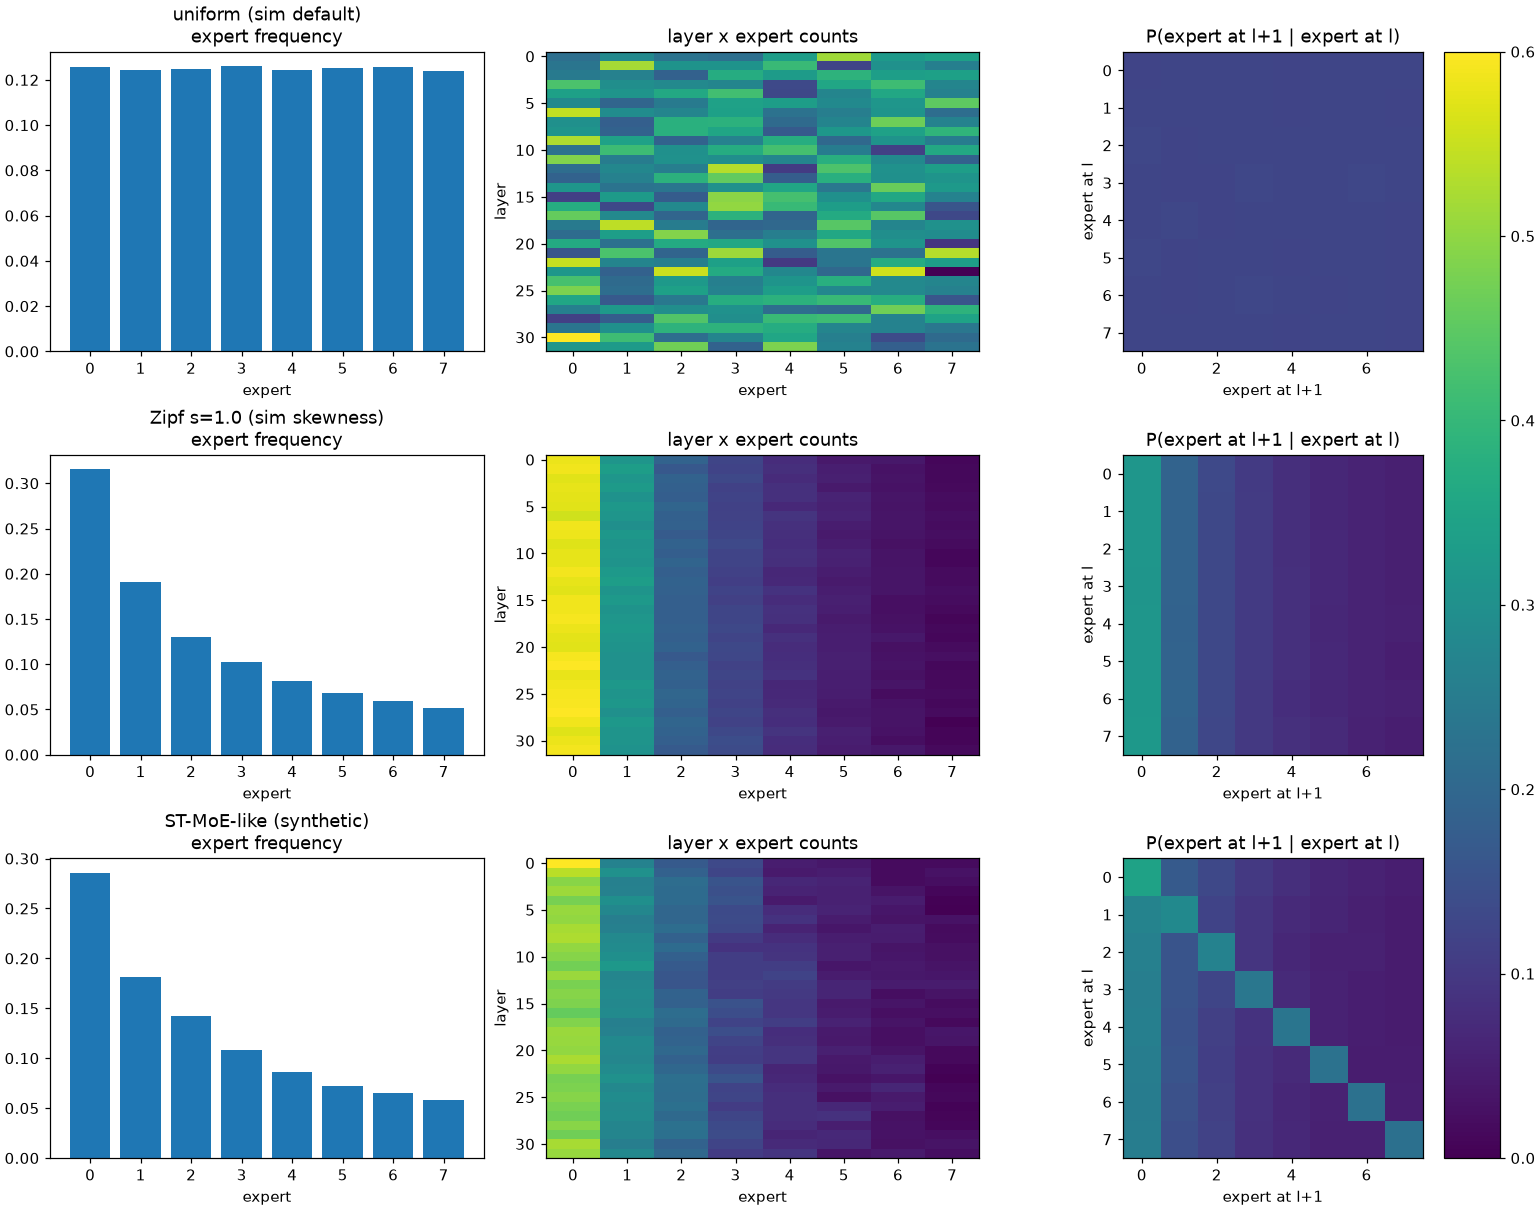
\includegraphics[width=\textwidth]{d4_correlation.png}
\caption{Generated by \texttt{analysis\_d4.py}: expert frequency, layer-by-expert counts and the transition matrix for each routing scenario. Only the correlated trace has a diagonal (predictable) transition matrix.}
\label{fig:d4}
\end{figure}

The overlap expected by pure chance is $2/8 = 0.25$; Figure~\ref{fig:d4} shows the same statistics as plots. Three things stand out:
\begin{itemize}
\item The simulator's routing has \textbf{no} correlation --- both overlaps sit on the 0.25 null and the transition matrix is flat. Any predictor we build must be evaluated on traces with real structure.
\item Zipf skew only concentrates traffic on hot experts (one expert takes 31.5\% of accesses, overlap rises to 0.36). The transition matrix shows vertical stripes --- \textit{popularity}, not \textit{predictability}.
\item Only the sticky trace gives a diagonal transition matrix and overlaps well above the null (0.556 layer-to-layer, 0.825 token-to-token) --- that diagonal is what prediction exploits.
\end{itemize}

The consequence for our prefetcher plans: correlation can tell us \textit{which} experts to fetch early, but it barely reduces \textit{how many} we must fetch --- coverage stays between 6.45 and 7.24 of 8 experts in every case.

\chapter{Discussion}
\label{ch:disc}

\section{What we learned}

The four results tell one story. Decode is bandwidth bound; expert weights are huge (352.3~MB each) and see only 1--3 tokens, so 96.2\% of decoder time is spent reading expert weights (D3). Moving those experts off-chip puts them behind a 900~GB/s link, and because the copy and the GPU's execution contend for HBM, execution is left with only 2452~GB/s --- which is what makes loading cost $2.72\times$ what execution costs (D2). A PIM die that shares the HBM removes that extra hop for the bandwidth-bound experts, and that is where the $3.10\times$ comes from (D1). Whether prefetching can hide the rest depends on routing correlation (D4), which the stock simulator does not have.

\section{Limitations}

\begin{itemize}
\item Both simulators are analytical: no DRAM timing, no contention, no queueing. The numbers are idealized bounds, not measurements from real hardware.
\item The D2 framework has no expert caching, so 68.13~ms is the pessimistic on-demand cost.
\item The D1 speed-up is a decode-only slice, the best case for Logic-PIM; a mixed prefill+decode workload would show less.
\item D4's correlated trace is synthetic. It validates our analysis, not real Mixtral routing --- real traces are needed before claiming any prediction accuracy.
\item The 900~GB/s off-chip link is a fast interconnect; a slower host would make loading dominate even more.
\end{itemize}

\section{Reproducibility}

Everything was regenerated from the files in the project folder: both simulators were rebuilt from scratch in a clean container, D1 and single-GPU logs came out byte-identical, the D2 columns reproduced exactly (one unused energy column drifted by $5\times10^{-8}$, a floating-point artifact), and all three analysis scripts exit 0. Build and run commands are in Appendix~\ref{app:cmds}.

\chapter{Conclusion and Future Work}
\label{ch:conc}

We reproduced Duplex and measured a $3.10\times$ decode speed-up, almost all of it from the Logic-PIM. We showed with a memory accounting that Mixtral-8x7B cannot fit in one 80~GiB GPU ($88.48 > 80$~GiB), so its experts must live in off-chip DRAM, and measured that loading the experts costs $2.72\times$ as much as executing them --- a ratio that reduces exactly to the leftover-bandwidth identity $(\text{HBM} - \text{link})/\text{link} = 2452/900$, because the copy consumes 900~GB/s of HBM while the GPU executes. From the operation tree we established where the decoder step spends its time: expert FFNs are 96.2\% of decoder time and one expert projection's weight read costs $98\times$ its arithmetic. Finally, we showed that the stock simulator's uncorrelated routing leaves nothing to predict, and that structure in the trace is what a prefetcher needs --- and that even then correlation changes \textit{which} experts to fetch, not \textit{how many}.

For the end-semester phase we plan to:
\begin{enumerate}
\item Implement a training-free expert predictor in the spirit of ST-MoE \cite{stmoe} and APEX \cite{apex}, and score it against the experts actually routed.
\item Build a prefetcher that fetches predicted experts into HBM ahead of use, overlapping loading with attention.
\item Compare with on-demand execution on latency, exposed stalls, extra traffic and energy.
\end{enumerate}

\begin{thebibliography}{9}

\bibitem{duplex}
S.~Yun et al., ``Duplex: A device for large language models with mixture of experts, grouped query attention, and continuous batching,'' arXiv:2409.01141 [cs.AR], 2024.

\bibitem{stmoe}
Y.~Zhao, R.~Bunescu, A.~Louri, A.~Karanth, and K.~Wang, ``A spatio-temporal expert prefetching framework for efficient MoE-based LLM inference,'' arXiv:2606.15453 [cs.AR], 2026.

\bibitem{apex}
A.~Kanani, L.~Badawi, and U.~Y.~Ogras, ``APEX: Adaptive expert prefetching for memory-efficient edge MoE inference,'' arXiv:2608.11688, 2026.

\bibitem{mixtral}
A.~Q.~Jiang et al., ``Mixtral of experts,'' arXiv:2401.04088, 2024.

\bibitem{roofline}
S.~Williams, A.~Waterman, and D.~Patterson, ``Roofline: An insightful visual performance model for multicore architectures,'' \textit{Communications of the ACM}, vol.~52, no.~4, pp.~60--67, 2009.

\bibitem{h100}
NVIDIA Corporation, ``NVIDIA H100 Tensor Core GPU architecture,'' whitepaper, 2022.

\bibitem{llmsim}
scale-snu, ``LLMSimulator,'' \url{https://github.com/scale-snu/LLMSimulator}.

\bibitem{ssd}
scale-snu, ``SSD-offloading,'' \url{https://github.com/scale-snu/SSD-offloading}.

\end{thebibliography}

\appendix

\chapter{Run Commands}
\label{app:cmds}

\begin{lstlisting}
cd ~/Downloads/CA_Project        # the project folder

# build (Ubuntu 22.04 container with g++-11, cmake, make, git)
cd LLMSimulator && mkdir -p build data && cd build && \
  cmake -DCMAKE_CXX_COMPILER=g++-11 -DCMAKE_C_COMPILER=gcc-11 -DCMAKE_CXX_STANDARD=17 .. && \
  make -j4
cd ../../SSD-offloading/LLMSimulator && mkdir -p build && cd build && \
  cmake -DCMAKE_CXX_COMPILER=g++-11 -DCMAKE_C_COMPILER=gcc-11 -DCMAKE_CXX_STANDARD=17 .. && \
  make -j4 run
cd ../../..                     # back to the project folder

# D1 + D2 OOM + D3 op tree
cd LLMSimulator/build && \
  ./run ../../mixtral_gpu.yaml        > ../../run_mixtral_gpu.log && \
  ./run ../../mixtral_duplex.yaml     > ../../run_mixtral_duplex.log && \
  ./run ../../mixtral_single_gpu.yaml > ../../run_mixtral_single.log

# D1 isolation: the same D1 configs with one field flipped each
#   mixtral_gpu.yaml with expert_tensor_degree/none_expert_tensor_degree = 4
#   mixtral_duplex.yaml with parallel_execution = off
# their logs and CSVs are kept in rerun_backup/

# D2 load vs exec (the SSD framework reads ./config.yaml from the CWD)
cd ../../SSD-offloading/LLMSimulator/build && \
  cp ../../../ssd_cfgs/cpu.yaml config.yaml      && ./run > ../../../ssd_results/ssd_cpu.log && \
  cp ../../../ssd_cfgs/cpu_copy.yaml config.yaml && ./run > ../../../ssd_results/ssd_cpu_copy.log && \
  cp tmp/*.csv ../../../ssd_results/
cd ../../..                     # back to the project folder

# analysis
python3 analysis_d2.py
python3 analysis_d3.py
python3 analysis_d4.py     # needs numpy + matplotlib, writes d4_correlation.png
\end{lstlisting}

\end{document}
